In this section we demonstrate the methods described so far and implemented in the software using a simple scenario. The network, shown in Figure \ref{fig:config}, has six links numbered 0 through 5. Links 0 through 4 have flow capacities of 2,000 veh/hour, while link 5 has a capacity of 1,000 veh/hour. All links except for link 2 are 200 meters in length. Link 2 is 400 meters. The free-flow speed in all links is 70 km/hr, and hence the free-flow travel time for all links except link 2 is about 10 seconds, while for link 2 it is about 20 seconds. There are two origin/destination pairs: OD 1, going from source node 0 to sink node 5, and OD 2, going from source node 1 to sink node 5. There are two paths available to OD 1: path 1, consisting of links [0, 3, 4, 5], and path 2 consisting of links [0, 2, 4, 5]. OD 2 is confined to path 3 = [1, 3, 4, 5]. Path [1, 2, 4, 5] is not utilized.

This network was chosen because it is small enough that the results are intuitive, and yet it illustrates the essential differences between the models and travel time functions described in Section~\ref{sec:models}. Only OD pair 1 has a choice of route, and hence the assignment problem is only to decide how the demand for OD 1 should be split between paths 1 and path 2 during each time interval. The total demand for both ODs will be set to a value that exceeds the capacity of link 5, and hence we expect congestion to form and propagate upstream past link 4, and onto to links 2 and 3, regardless of the assignment. Because path 1 is shorter than path 2, OD 1 should choose path 1 until the accumulated congestion on link 3 causes its travel time to be as large or larger than that of link 2. Then the assignment should distribute traffic on paths 1 and 2 such that the travel times on links 2 and 3 are equalized. 

\begin{figure}[h]
    \centering
    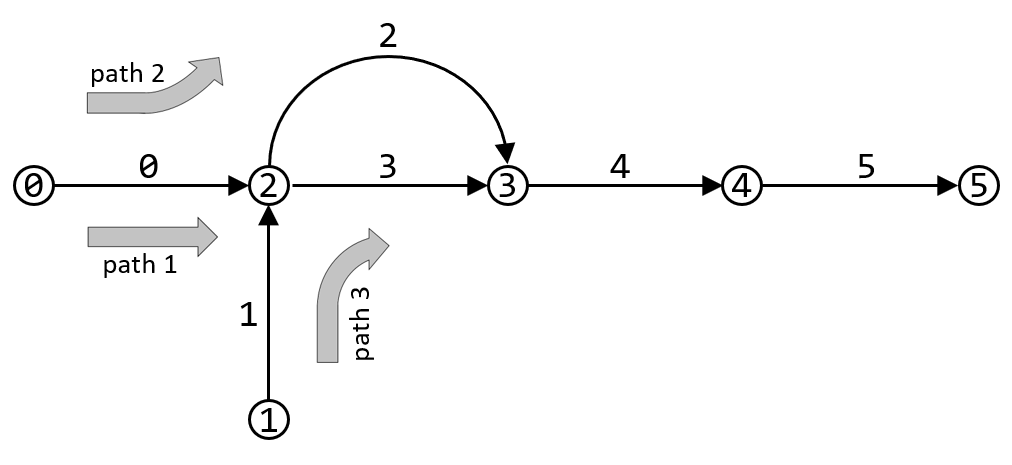
\includegraphics[width=\linewidth]{figs/config.png}
    \caption{Traffic network.}
    \label{fig:config}
\end{figure}

\subsection{Static assignment}
The static assignment problem with BPR cost function is the simplest case of traffic assignment. It can be posed as a convex optimization problem and solved efficiently with the Frank-Wolfe procedure. Figure~\ref{fig:static} shows solutions obtained with OD demands set to $d_0$=1300 veh/hr, $d_1$=300 veh/hr, and $\gamma$ ranging from 0 to 20. Equilibria with $h_1\neq 0$ and $h_2\neq 0$ are characterized by $\tau_2=\tau_3$. Using Eq.~\ref{eq:bpr}), feasibility ($h_1+h_2=d_0$ and $h_3=d_1$), and $\tau^0_2=2\;\tau^0_3$, this leads to,
\begin{equation}
\bar{f}^4 + \gamma\left(\;2(d_0-h_1)^4 - (d_1+h_1)^4 \;\right) = 0
\end{equation}
\todo[inline]{what is $\gamma$? Seems to not have been define, Juliette}
The root locus method \cite{rootlocus} can be applied here to track the trajectory of real solutions of this equation for $\gamma$'s ranging from zero to infinity.

% See Figure~\ref{fig:rlocus}. 
In the limit as $\gamma\rightarrow\infty$, the equilibrium value of $h_1$ decreases to 569.14 (the smallest real root of $2(d_0-h_1)^4 - (d_1+h_1)^4$), and $h_2=1300-h_1$ increases to 730.86. Thus, paradoxically, for $\gamma$ larger than a threshold, the number of vehicles that choose path 2 exceed those that choose path 1, even though path 2 is longer than path 1. This observation should be seen as a shortcoming of the BPR function as a model of travel time.

\begin{figure}[h]
    \centering
    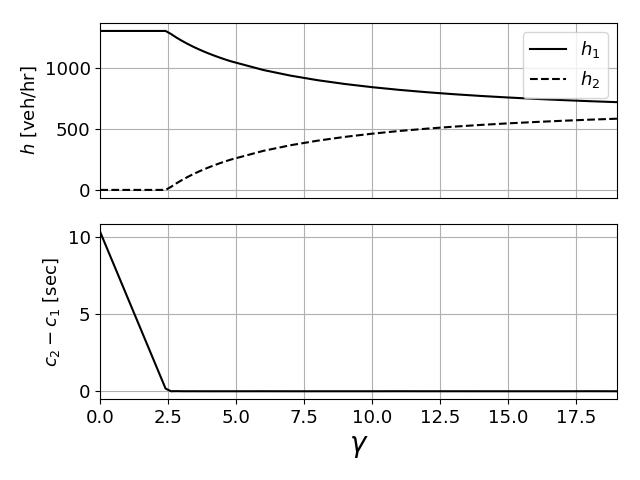
\includegraphics[width=0.8\linewidth]{figs/static.png}
    \caption{Static equilibria as a function of $\gamma$.}
    \label{fig:static}
\end{figure}

% \begin{figure}[h]
%     \centering
%     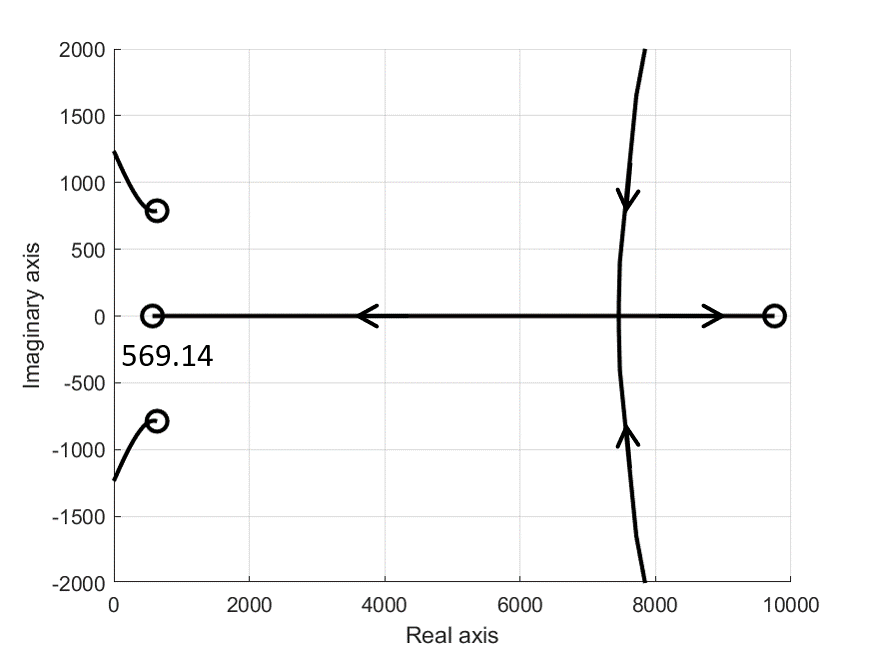
\includegraphics[width=0.8\linewidth]{figs/rlocus_mod.png}
%     \caption{Root locus.}
%     \label{fig:rlocus}
% \end{figure}

\subsection{Dynamic assignment}
Next we compute the dynamic equilibrium assignments under three different models: the MN model, the CTM model with instantaneous travel time, and the CTM with predictive travel time. The time period is 600 seconds. Demands are set to $d_0$=1300 and $d_1$=300 for time $\in[0,300]$ seconds, and $d_0$=$d_1$=0 thereafter. EPM was used to compute the solution, with an initial guess provided by MSA. The three solutions are shown in Figure~\ref{fig:ctm_vs_mn_hc}. The optimal assignment under the MN model places all of $d_0$ on path 1 for all times before 300 seconds, and so link 2 remains unused. This is because MN does not propagate congestion upstream, and so link 3 never slows down. This can be seen in Figure~\ref{fig:ctm_vs_mn_x}, where link 4 accumulates vehicles without bound up to 300 seconds. 
\begin{figure}[h]
    \centering
    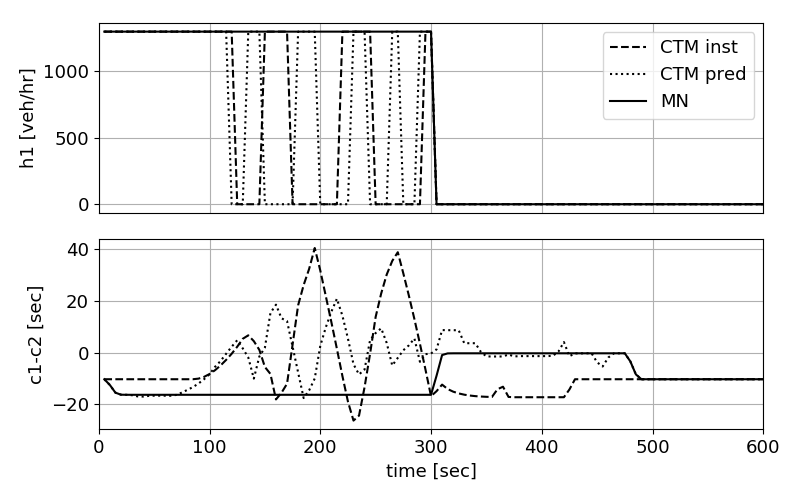
\includegraphics[width=\linewidth]{figs/ctm_vs_mn_hc.png}
    \caption{ctm vs mn hc}
    \label{fig:ctm_vs_mn_hc}
\end{figure}

\begin{figure}[h]
    \centering
    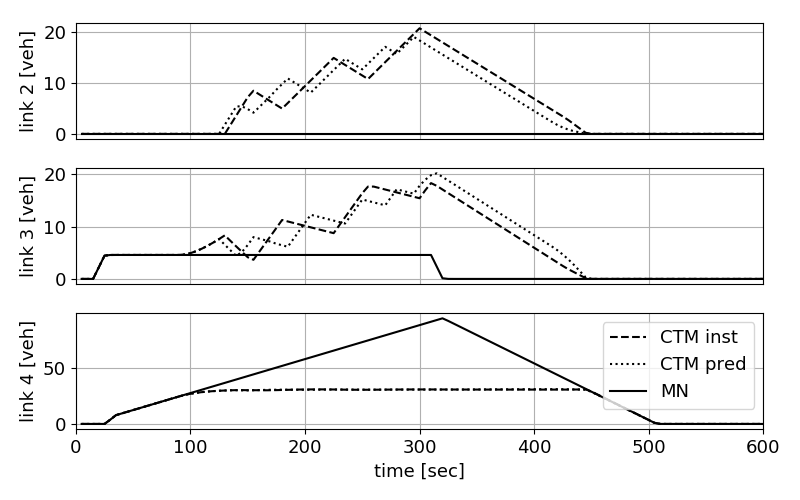
\includegraphics[width=\linewidth]{figs/ctm_vs_mn_x.png}
    \caption{ctm vs mn x}
    \label{fig:ctm_vs_mn_x}
\end{figure}
The two CTM solutions display behavior that is more realistic. In both cases, the entire demand is initially sent on path 1, since $c_2-c_1$ is positive, as can be seen in Figure~\ref{fig:ctm_vs_mn_hc}. The congestion on link 4 spills to link 3 after around 100 seconds, and at this point $c_2-c_1$ begins to decrease. Notice that the predictive version of travel time reacts before congestion reaches link 3. The travel times on paths 1 and 2 are equalized at around 116 seconds for CTM predictive, and 121 seconds for CTM instantaneous. At this point, the demand is shifted entirely to path 2. The effect of this change is delayed by the travel time on link 0. In the meantime, $c_1$ continues to increase, and hence $c_2-c_1$ becomes negative. After the pulse reaches links 2 and 3, the travel time on path 1 decreases rapidly, and travel time on path 2 increases. $c_2-c_1$ again becomes positive, and another oscillation begins. 

\begin{figure}[h]
    \centering
    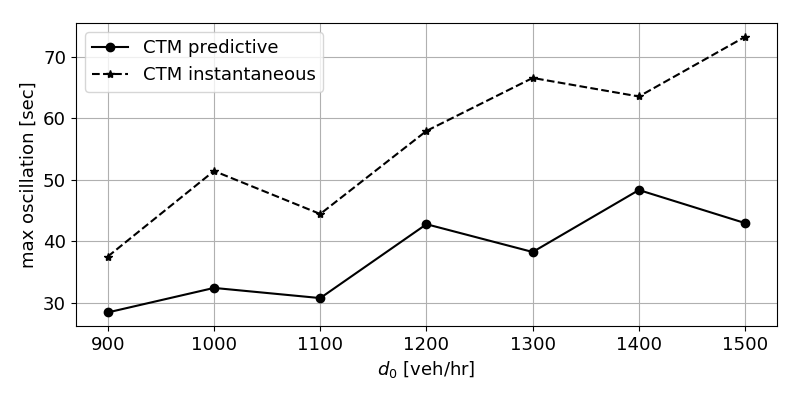
\includegraphics[width=0.8\linewidth]{figs/peaks.png}
    \caption{peaks }
    \label{fig:peaks}
\end{figure}

An immediate question is whether these oscillations are realistic. We do not attempt here to answer this question, but limit ourselves to a quantification of their size. Figure~\ref{fig:peaks} shows the maximum difference between consecutive peaks and valleys observed in the equilibrium assignment for a range of values for $d_0$ (from 900 vph to 1500 vph). Notice that the maximum oscillation with predictive travel time is uniformly smaller than that with instantaneous travel time. It is not clear to us at this point whether these oscillations are a property of the equilibrium solutions, a consequence of the discretization scheme, or related to the numerical solution methods. 

\begin{figure}[h]
    \centering
    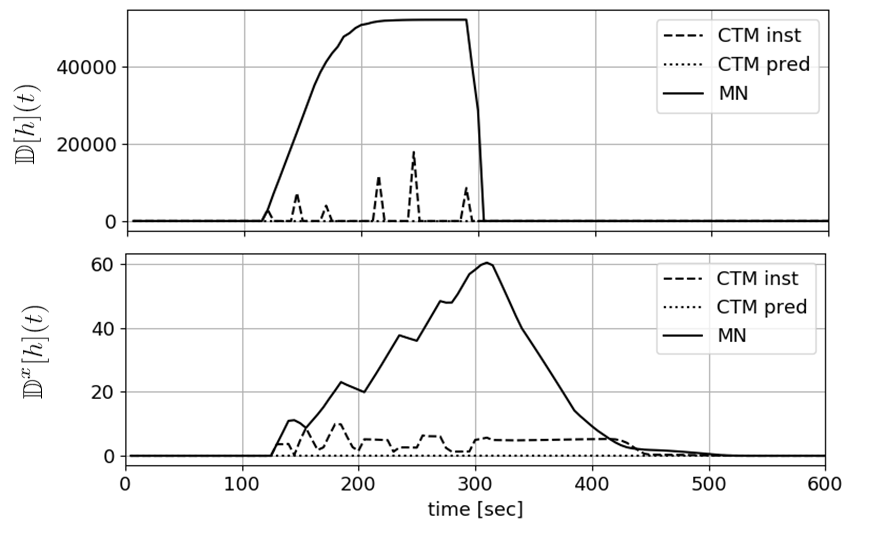
\includegraphics[width=\linewidth]{figs/DWardrop.png}
    \caption{DWardrop}
    \label{fig:dWardrop}
\end{figure}

% \begin{figure}[h]
%     \centering
%     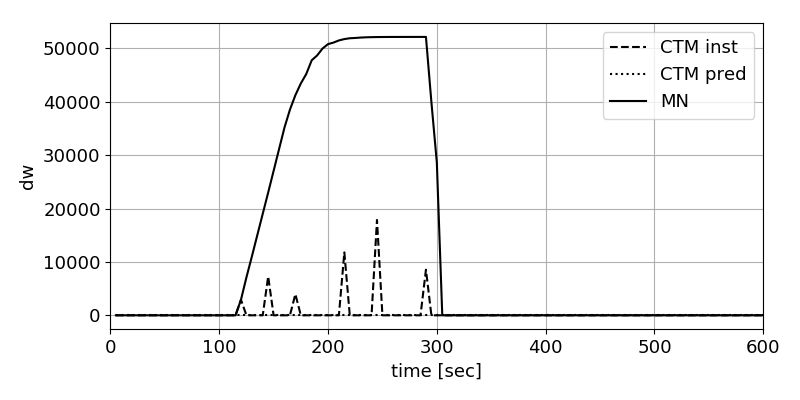
\includegraphics[width=\linewidth]{figs/dw.png}
%     \caption{dw}
%     \label{fig:dw}
% \end{figure}

Finally, we evaluate these three solutions in terms of their similarity to a Wardrop user equilibrium. To build a `distance to Wardrop' function, we express Wardrop's principle as a complementarity condition: $h^*$ is an equilibrium  if it is feasible and for all time $t$, all OD pairs $w$, and all paths $p\in\mathcal{P}_w$,
\begin{equation}
\label{eq:comp}
h_p(t)\left(c_p(t)-\pi_w(t)\right) = 0
\end{equation}
where $\pi_w(t)$ is the minimum travel time among paths in $\mathcal{P}_w$. The left hand side of Eq. (\ref{eq:comp}) is positive for all feasible assignments, and zero only for equilibrium assignments. Therefore the function,
\begin{equation}
\mathbb{D}[h](t) =\sum_w \sum_{p\in\mathcal{P}_w} h_p(t)\left(c_p(t)-\pi_w(t)\right)
\end{equation}
can serve as a rough measure of `distance to Wardrop', although it does not satisfy the triangle inequality nor the uniform scaling requirements of a norm. Computation $\mathbb{D}[h](t)$ requires a model to provide the travel times $c_p(t)$ corresponding to $h$. Here we use the CTM with predictive travel time, since it is the model that most closely matches our intuitions about the outcomes of the experiment. The results are shown in Figure~\ref{fig:dWardrop}. Clearly the equilibrium due to the MN model is farther from a Wardrop equilibrium than either of the CTM results. A shortcoming of $\mathbb{D}[h](t)$ is that it only penalizes incorrect assignments $h(t)$ at time $t$. The lingering effects of vehicles sent on non-minimum paths are lost. If, however, the problem has a unique equilibrium solution, then the distance to that state trajectory can also be used to measure `distance to Wardrop'.
\begin{equation}
\mathbb{D}^x[h](t) = \sum_{l} ||x^{*}(t)-x(t)||
\end{equation}
Here, $x^{*}(t)$ and $x(t)$ are, respectively, the equilibrium state trajectory and the state trajectory due to $h$. This quantity is depicted in the lower plot of Figure~\ref{fig:dWardrop}. Notice that the error persists beyond $t$=300.